\documentclass[12pt]{article}

\usepackage{fullpage}
\usepackage[round]{natbib}
\usepackage{multirow}
\usepackage{booktabs}
\usepackage{graphicx}
\usepackage{float}
%\usepackage{../ltx/edcomms}
\usepackage{hyperref}
\usepackage{geometry}
\usepackage{changepage}
\usepackage{adjustbox}
\usepackage{graphicx}
\usepackage[section]{placeins} % Prevents floats from floating across sections
\newcounter{acnum}
\newcommand{\actheacnum}{AC\theacnum}
\newcommand{\acref}[1]{AC\ref{#1}}

\newcounter{ucnum}
\newcommand{\uctheucnum}{UC\theucnum}
\newcommand{\uref}[1]{UC\ref{#1}}

\newcounter{mnum}
\newcommand{\mthemnum}{M\themnum}
\newcommand{\mref}[1]{M\ref{#1}}

\begin{document}

\title{\vspace*{3cm} Module Guide for ECA Rules for Ampersand} 
\author{Yuriy Toporovskyy,\ Yash Sapra,\ Jaeden Guo}
\date{February 13th,\ 2016} 

	
\maketitle
\vspace*{1cm}
\begin{table}[ht!]\begin{center}
        \caption{Revision History}  
        \begin{tabular}{|c|c|c|}\hline
            \textbf{Author} & \textbf{Date} & \textbf{Comment} \\\hline 
            Yash Sapra & 24 / 02 / 2016 & Initial draft\\\hline
        \end{tabular}
    \end{center}\end{table}
\newpage

\tableofcontents

\newpage

\section{Introduction}
%TODO: edit for grammar, spelling, context, flow, watch for contractions
\subsection{Description}
The document outlines the design decision for the EFA project. 
EFA is responsible for generating SQL from ECA rules that will 
be used to fixed any data inconsistencies in the Ampersand Database.

This document follows the principle set by Parnas and Clements \citep{fakeIt} . 
Ampersand is currently in development where modifications are frequent, a 
commonly accepted practice for this situation is to decompose modules based on 
the principle of abstraction, where unnecessary information in hidden for the 
benefit of designers and maintainers\citep{modStruct,Parnas1972}.
 
Our design follows the principles layed out by \citep{modStruct}, as follows:
\begin{itemize}
\item Unnecessary design details are omitted for simplicity
\item Each data structure is only in one module
\item Any other program that requires information stored in a module's data
  structures must obtain it by calling access programs belonging to that module.
Additionally: 
\item Each module is broken down based on hierarchy
\item Reference material are provided for external libraries but details of its 
use will not be provided within the module break-down
\end{itemize}

\subsection{Scope}
This project aims to improve upon the current Ampersand system by providing a 
permanent replacement for the exec-engine. EFA automatically restores system 
invariants according to ECA rules with no manual maintenance required.

\subsubsection{Intended Audience}
This document is designed for:
\paragraph{New project members:}
This document designed to be a guide to introduce new Ampersand users to EFA 
(ECA rules for Ampersand). It provides a basic structure that allows 
individuals to quickly access what they are looking for.
   
\paragraph{Maintainers \& Designers:} The structure of this module guide will 
help maintainers rationalize where changes should be made in order to 
accomplish their intended purpose. Furthermore, the design document will act as 
a guide to EFA for future designers of Ampersand.

\section{Anticipated and Unlikely Changes}
\subsection{Anticipated Changes}
It is likely that EFA will require changes to the front-end interface and an 
addition that integrates the front end to the back-end. Furthermore, the number 
of ECA rules are not permanent and if changes are made to the ECA rules, those 
changes will need to be incorporated into EFA. 

Thus far anticipated changes include:

\begin{description}
    \item[AC1:] New front-end interface.
    \item[AC2:] Addition or elimination of ECA rules.
    \item[AC3:] The algorithm used for EFA.
    \item[AC4:] The format of output.
    \item[AC5:] The format of input parameters.
    \item[AC6:] The format of initial input data and associated markers for 
    data association.
    \item[AC7:] Integration of front-end interface to back-end modules.
    \item[AC8:] Implementation of SQL data structure
    \item[AC9:] Testing for individual modules and internal systems
    \item[AC10:] Software requirements for running Ampersand and by extension 
    EFA
    
\end{description}

\subsection{Unlikely Changes} 

These unlikely changes include the things that will remain unchanged in the 
system, and also changes that would not affect EFA. 

\begin{description}
    \item[UC1:] There will always be a source of input data external to the 
    software. 
    \item[UC2:] Results will always be provably correct. 
    \item[UC3:] The goal of EFA is to automatically correct system invariants
    \item[UC4:] Output data must exist
    \item[UC5:] The implementation language must be the same as that which is 
    used for building the Ampersand system
    \item[UC6:] The format of initial input data and associated markers for 
    data association. 
    \item[UC7:] Type of output data will always be SQL.
\end{description}

\section{Use Hierarchy \& Dependency Graph }
This section provides an overview of the module design. Modules are decomposed 
based on their hierarchy from top to bottom. The modules are broken down into 
two sections, the first section consists of the main modules used for EFA, the 
second section contains support module and finally the last sections contain 
external libraries.

\begin{figure}
    \centering
    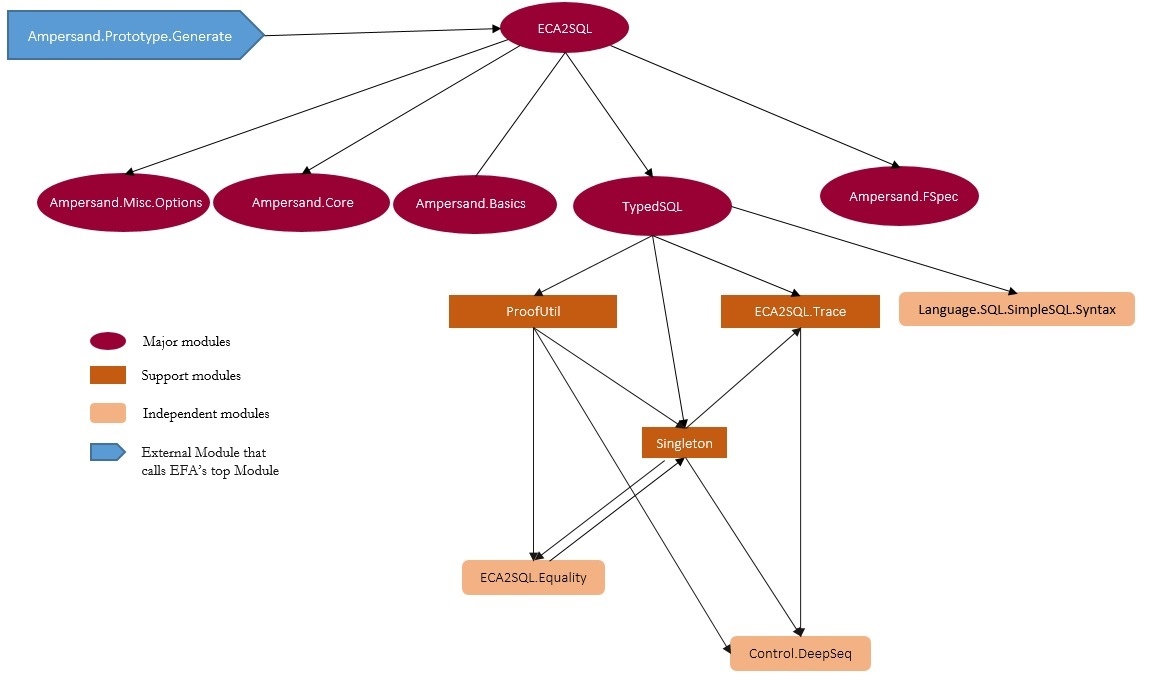
\includegraphics[width=0.95\textwidth]{../DesignDoc/depent_tree}
    \caption{Dependency graph of EFA modules}~\label{fig:figure1}
\end{figure}


\section{Main Modules}

\section{Support Modules}

\section{External Libaries}

\section{Connection Between Requirements and Design} \label{SecConnection}


\section{Module Decomposition} \label{SecMD}

\section{Behaviour-Hiding Module}

\section{Software Decision Module}

\section{Traceability Matrix} \label{SecTM}

\section{Use Hierarchy Between Modules} \label{SecUse}



%\section*{References}

\bibliographystyle {plainnat}
\bibliography {docDesign}

\end{document}